\scanpage{21}
\mspage{20}\mspage{10}
\figure{\begin{tikzpicture}\node[draw,ellipse] {$\overline{\underline{\mathrm{VI}}}$};\end{tikzpicture}}
\margin{\uline{Relation with field structure}}
Let us forget the topological structures, suppose on the other hand that $R$ has a \uline{field structure}. We shall then assume, \deleted{\unsure{Alrt}} in addition to $(M1)_{\unsure{0}}$ and $(M4)$ (minimum for constructing $\operatorname{Esp}_{\mathcal M_*}$ with its finite $\varprojlim$) the axiom

\deleted{$(M11)$ \deleted{a) For every} tame subset $A$ of $R$, the map $a\mapsto-a$ from $A$ to $R$ is tame (i.e. the set $\{(a,-a)\in R^2\mid a\in A\}$ is \unsure{tame|tame})}

\figure{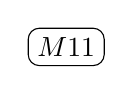
\begin{tikzpicture}\node[draw,rounded corners] {$M11$};\end{tikzpicture}}
a) $0$ and $1$ are $\in R_0$ i.e. $\{0\},\{1\}\in\mathcal M_1$

b) $\forall A\in\mathcal M_2$, the functions
\[
 (x,y)\longmapsto x-y\qquad
 (x,y)\mathrel{\mapstochar\relbar}xy
\]
\deleted{c) $\forall A\subset R^*$, $A\in\mathcal M_1$, $\exists B\in\mathcal M_1$ such that $A^{-1}\subset B$}
\margin{\deleted{(\unsure{for|we may assume} we may assume $B=A^{-1}$\,!)}}
on $A$ are tame, \deleted{\unsure{for}} i.e. the two subsets of $R^3$
\[
 \{(x,y,x-y)\mid(x,y)\in A\},\qquad\text{and }\{(a,y,xy)\mid(x,y)\in A\}
\]
are tame.

c) $\forall A\subset R^*$, $A\in\mathcal M_1$, $\exists B\in\mathcal M_1$ with $A^{-1}$ \deleted{tame}\inserted{$\subset B$} (we may assume $B=A^{-1}$\,!).

\deleted{This axiom} \deleted{\unsure{the parts a) b)}} \inserted{the parts a) b)} \unsure{are equivalent|is equivalent} to the validity of the

\margin{\uline{NB} If $R\in\mathcal M_1$, it suffices to take $(M11)$ for $A=R^2$}

\uline{Proposition} For a tame space $X$, the tame functions $X\mathbin{-}R$ \deleted{\unsure{and|is} = a sub $R_0$} form a \uline{subring} of the ring of scalar functions on $X$. In particular, $R_0$ is a subring of $R$, and the rings
\margin{of tame functions are $R_0$-algebras}
